\documentclass{standalone}
    \usepackage{tikz}
    \usetikzlibrary{patterns}
    \usepackage{pgfplots}
    \pgfplotsset{compat=1.10}
    \usepgfplotslibrary{fillbetween}
    \begin{document}
    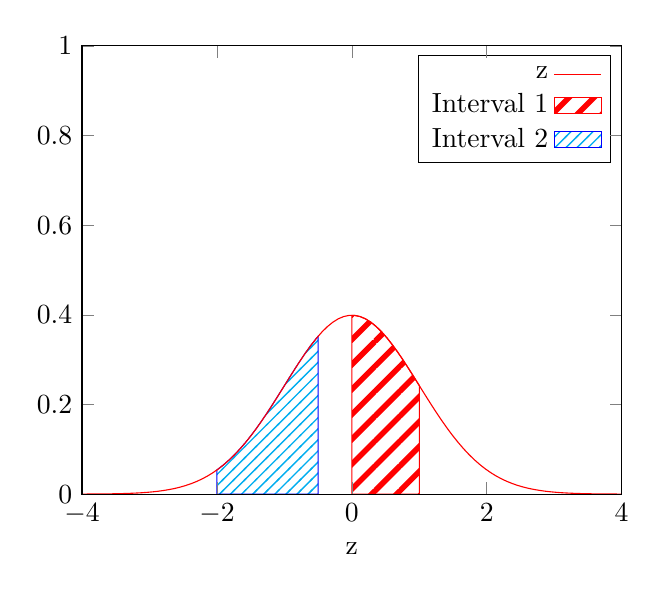
\begin{tikzpicture}
    \tikzset{
        hatch distance/.store in=\hatchdistance,
        hatch distance=10pt,
        hatch thickness/.store in=\hatchthickness,
        hatch thickness=2pt
    }

    \makeatletter
    \pgfdeclarepatternformonly[\hatchdistance,\hatchthickness]{flexible hatch}
    {\pgfqpoint{0pt}{0pt}}
    {\pgfqpoint{\hatchdistance}{\hatchdistance}}
    {\pgfpoint{\hatchdistance-1pt}{\hatchdistance-1pt}}%
    {
        \pgfsetcolor{\tikz@pattern@color}
        \pgfsetlinewidth{\hatchthickness}
        \pgfpathmoveto{\pgfqpoint{0pt}{0pt}}
        \pgfpathlineto{\pgfqpoint{\hatchdistance}{\hatchdistance}}
        \pgfusepath{stroke}
    }

    \begin{axis}[
        xmin=-4,xmax=4,
        xlabel={z},
        ymin=0,ymax=1,
        axis on top,
        legend style={legend cell align=right,legend plot pos=right}] 

    \addplot[name path=A,color=red,domain=-4:4,samples=100] {1/sqrt(2*pi)*exp(-x^2/2)};
    \addlegendentry{z}

    \path[name path=B] (axis cs:\pgfkeysvalueof{/pgfplots/xmin},0) -- (axis cs:\pgfkeysvalueof{/pgfplots/xmax},0);

    \addplot+[draw,pattern=flexible hatch,pattern color=red]
    fill between[
        of=A and B,
        soft clip={domain=0:1},
    ];
    \addlegendentry{Interval 1}

    \addplot[pattern=flexible hatch,pattern color=cyan,draw=blue,hatch distance=5pt, hatch thickness=0.5pt]
    fill between[
        of=A and B,
        soft clip={domain=-2:-0.5},
    ];
    \addlegendentry{Interval 2}
    \end{axis}
\end{tikzpicture}
\end{document}
